% proposal.tex: short case for merging parts of the fork EdoardoBonetti/ngsolve into NGSolve master (GitLab).
% Numbers: results/musica/*.json (musica/sweep_ab.py) and results/*.json (Mac, tests_ab.py); figure and table:
% python3 ../plot_sweep.py. Build: latexmk -pdf proposal.tex
\documentclass[10pt,a4paper]{article}
\usepackage[margin=1.7cm,top=1.5cm,bottom=1.6cm]{geometry}
\usepackage{fontspec}
\usepackage{unicode-math}
\setmainfont{TeX Gyre Pagella}
\setmathfont{TeX Gyre Pagella Math}
\usepackage{booktabs,tabularx,array,graphicx,xcolor,enumitem,microtype}
\newcolumntype{Y}{>{\raggedright\arraybackslash}X}
\usepackage[hidelinks]{hyperref}
\definecolor{tu}{HTML}{1f5fa8}
\setlist{nosep,leftmargin=1.2em}
\setlength{\parindent}{0pt}\setlength{\parskip}{4pt}
\newcommand{\sect}[1]{\par\vspace{5pt}{\large\bfseries\color{tu}#1}\par\vspace{1pt}}
\pagestyle{empty}

\begin{document}
{\LARGE\bfseries From the fork to NGSolve master: what to merge, and why}\\[2pt]
Edoardo Bonetti \hfill \today

\vspace{-2pt}
\textbf{In short.} The fork (\href{https://github.com/EdoardoBonetti/ngsolve}{\texttt{EdoardoBonetti/ngsolve}},
branch \texttt{ngsolve}, merged with master \texttt{6e701b568} on 9 November) holds
\textbf{12 fixes for bugs in current master}, each with a regression test that fails on master, and
\textbf{six changes measured at three problem sizes}: four are faster at every size, two from medium size on.
Each change is a separate small merge request of cherry-picked
commits; all but three apply to master without conflicts.

\sect{1\quad Speed: upstream master against the fork, small / medium / large}
Both builds compiled with identical options (Release, UMFPACK, CPU only) on MUSICA; all runs on one
AMD Zen\,4 node (48 cores, 192\,GB); each upstream/fork pair runs back to back in the same job. Times are wall times
of the operation itself; every fork result agrees with upstream (matrix norms, eigenvalues, traced
length, interpolation errors).

\begin{center}\small
\begin{tabularx}{\textwidth}{@{}>{\raggedright\arraybackslash}X ccc@{}}
\toprule
& \textbf{small} & \textbf{medium} & \textbf{large}\\
\midrule
Field lines & 0.774 $\to$ 0.0137 s, \textbf{56$\times$} & 5.45 $\to$ 0.0747 s, \textbf{73$\times$} & 75.2 $\to$ 0.976 s, \textbf{77$\times$} \\
H1 transfer (\texttt{localhoprolongation}) & 0.00839 $\to$ 0.00476 s, \textbf{1.8$\times$} & 0.162 $\to$ 0.103 s, \textbf{1.6$\times$} & 1.09 $\to$ 0.605 s, \textbf{1.8$\times$} \\
Eigenvalues (GPLHR + MG vs Arnoldi + UMFPACK) & 2.1 $\to$ 2.62 s, \textbf{0.80$\times$} & 15.1 $\to$ 7.18 s, \textbf{2.1$\times$} & 135 $\to$ 21.7 s, \textbf{6.2$\times$} \\
SIMD edge forms & 0.00686 $\to$ 0.00419 s, \textbf{1.6$\times$} & 0.032 $\to$ 0.0256 s, \textbf{1.2$\times$} & 0.185 $\to$ 0.132 s, \textbf{1.4$\times$} \\
Complex system: real BDDC vs best complex BDDC & 0.045 $\to$ 0.0532 s, \textbf{0.85$\times$} & 0.373 $\to$ 0.341 s, \textbf{1.09$\times$} & 7.11 $\to$ 4.59 s, \textbf{1.5$\times$} \\
\texttt{mesh.Refine} & 1.01 $\to$ 0.963 s, \textbf{1.05$\times$} & 11.1 $\to$ 10.6 s, \textbf{1.05$\times$} & 121 $\to$ 116 s, \textbf{1.05$\times$} \\
\bottomrule
\end{tabularx}

\end{center}
\vspace{-4pt}
{\footnotesize Sizes (small/medium/large): field lines 500/2\,000/10\,000 lines on 6\,k/47\,k/379\,k tets;
H1 $p=4$ transfer to 0.14/2.3/14.3\,M dofs; eigenproblem H1 $p=2$ with 20/83/287\,k dofs; edge form VectorH1 $p=3$
with 18/137/987\,k dofs; complex system H1 $p=3$ with 9/63/443\,k dofs; \texttt{Refine} to 3.2/20/154\,M tets.}

\begin{center}
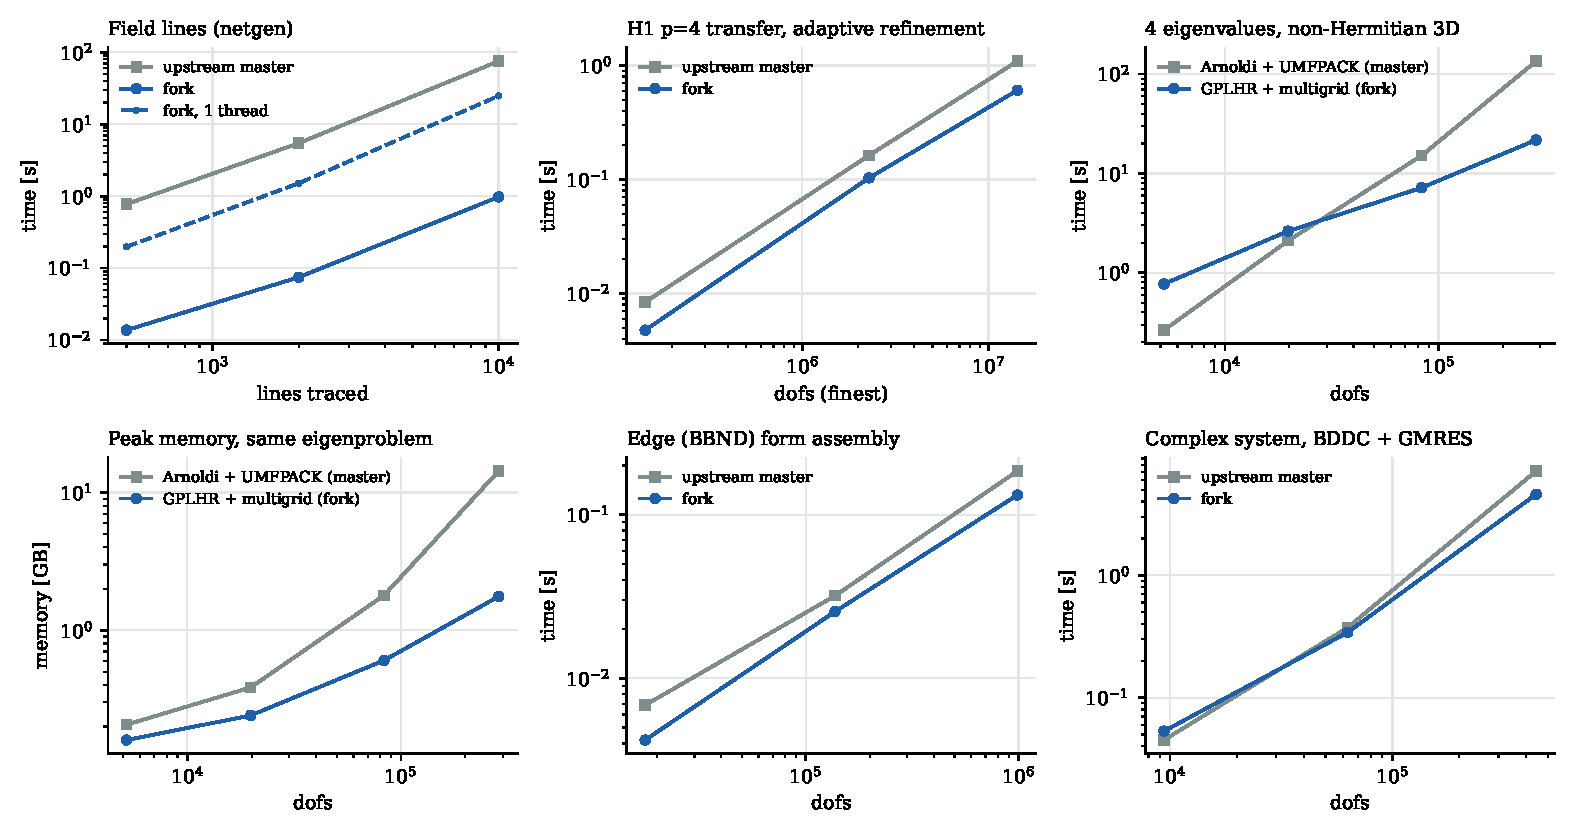
\includegraphics[width=\textwidth]{fig_sweep.pdf}
\end{center}
\vspace{-6pt}
{\small
\begin{itemize}
\item \textbf{Field lines} (netgen \texttt{FieldLineCalc}): testing the previous element before the search tree gives
  3--4$\times$ on one thread; the lines are independent and now run in parallel (25$\times$ more on 48 threads).
  Same traced length; 3.6\,\% more segments, because master carries the RK step size from one line into the next.
\item \textbf{H1 transfer}: cost proportional to the refined elements; memory 2.4\,$\to$\,1.3\,GB at 14.3\,M dofs;
  equal to \texttt{hoprolongation} to $10^{-14}$.
\item \textbf{Eigenvalues} of $-\Delta u + b\cdot\nabla u = \lambda u$ (unit cube, $b=(8,6,4)$): both return 58.61 and
  the triple 88.22. GPLHR needs only products with $A$, $M$ and a preconditioner; with geometric multigrid it wins from
  about 30\,k dofs and needs less memory at every size (14.6\,$\to$\,1.8\,GB at 287\,k). Below that, a direct solver
  is hard to beat (5\,k dofs: 0.26 vs 0.77\,s). At $p=2$, BDDC is no help: its wirebasket is the whole space.
\item \textbf{Complex systems}: master cannot apply a real preconditioner to a complex vector (Section 2), so it needs a
  complex BDDC. The fork's real BDDC: same iterations (16/17/19), 28\,\% less memory and 1.5$\times$ faster at
  443\,k dofs; equal on small problems (0.05\,s).
\item \textbf{SIMD edge forms}: identical matrices. \textbf{\texttt{mesh.Refine}}: 4--5\,\% at every size, a side benefit.
\end{itemize}}

\clearpage
\sect{2\quad Bugs in current master, fixed in the fork (one test each)}
\begin{center}\small
\begin{tabularx}{\textwidth}{@{}l Y r@{}}
\toprule
\textbf{Where} & \textbf{Symptom on master \texttt{6e701b568}} & \textbf{failing tests}\\
\midrule
\texttt{ComputeNormalAndMeasureET} & SIMD edge tangent is 0 (since the 3 Nov rework): BBND forms with \texttt{specialcf.tangential} assemble to zero & 1/3\\
\texttt{EdgeFaceTangentialVectors} & no SIMD evaluation: the integrator falls back to scalar code for good & 1/2\\
\texttt{u.Other(bnd=g)} & boundary-facet term missing from the assembled matrix & 2/2\\
\texttt{IntegrationRuleSpace.Set} & order $\ge 6$ in 3D: SIMD blocks of 64 points land on the wrong dofs (garbage, NaN) & 6/6\\
\texttt{Compile(...)} & with \texttt{code\_uses\_equivalence\_keys}: the generated C++ does not compile & 1/1\\
periodic \texttt{.Other()} & evaluated at wrong points when the identification reorders vertex numbers & 4/8\\
periodic \texttt{Set(dual=True)} & cached duality inverse picked from unrenumbered vertices (sent as GitHub PR \#102) & 8/10\\
L2 \texttt{hoprolongation} & spaces created after \texttt{Refine}: L2 error $10^{-5}\to 9\cdot10^{-2}$ & 8/15\\
\texttt{MultiVector.Orthogonalize()} & without \texttt{ipmat}: not orthonormal from 4 vectors on (block coupling used transposed) & 30/64\\
\texttt{DeviceCG}, \texttt{DeviceTFQMR} & NaN after exact convergence between residual checks & 5/7\\
real BDDC $\times$ complex vector & raises ``illegal combination of scalar types'': no real preconditioner for complex systems & 1/6\\
netgen \texttt{SplitAlfeld} & 3D split vertex outside the tet: inverted elements & 1/3\\
\bottomrule
\end{tabularx}
\end{center}

\sect{3\quad MPI: what carries over, pros and cons}
Assessment from the code; none of it is measured with MPI yet.
\begin{center}\small
\begin{tabularx}{\textwidth}{@{}l Y@{}}
\toprule
\textbf{Change} & \textbf{With MPI-distributed meshes}\\
\midrule
bug fixes, SIMD edge forms & element-local or vector-local: work unchanged on every rank.\\
real operator on complex vector & written through \texttt{BaseMatrix} with the operator's own real \texttt{ParallelDofs}
  (\texttt{parallelvvector.cpp} is covered); needs an \texttt{np}\,$\ge 2$ test.\\
GPLHR & needs only products with $A$, $M$, a preconditioner and inner products, so it should run on
  \texttt{ParallelMatrix} without changes. The preconditioner changes: BDDC ($p\ge3$) or hypre BoomerAMG, since geometric
  multigrid is shared-memory only. Arnoldi with shift-invert would need MUMPS, whose memory grows with the fill-in.\\
\texttt{localhoprolongation} & per-element formulas; needs the parent relation on each rank after parallel refinement.\\
field lines & thread-parallel only; lines cross subdomain borders, so they stay on one rank.\\
\bottomrule
\end{tabularx}
\end{center}
\vspace{-3pt}
\textbf{Pros of going MPI.}
\begin{itemize}
\item Memory: Arnoldi + UMFPACK already needs 14.6\,GB at 287\,k dofs, and a direct solver's memory grows faster
than the problem. With GPLHR and a distributed preconditioner, the memory is spread over the nodes.
\item GPLHR is the eigensolver that fits MPI: no global factorization, the same Python code on every rank.
\item The element-local fixes need no extra work, so MPI users get them for free.
\end{itemize}
\textbf{Cons.}
\begin{itemize}
\item On one node, threads already scale (field lines 25$\times$ from 1 to 48 threads at 10\,000 lines); MPI pays off only beyond one node's memory.
\item Build and test cost: MPI build with \texttt{mpi4py} and MUMPS or hypre, and an \texttt{np}\,$\ge2$ test in the CI for every change.
\item Adaptive refinement and geometric multigrid on distributed meshes are the least mature parts (load balance
  after refinement), so the \texttt{localhoprolongation} and multigrid gains do not transfer directly.
\end{itemize}

\sect{4\quad Proposed merge requests (GitLab, cherry-picked, smallest first)}
\begin{enumerate}
\item The bug fixes of Section 2, one MR each with its test (no API change).
\item SIMD edge forms: \texttt{EdgeFaceTangentialVectors} SIMD + tangential fix (needs a small rebase on the 3 Nov rework).
\item \texttt{H1(localhoprolongation=True)}, and prolongations for HCurlCurl and refined L2 spaces.
\item Real operators on complex vectors (\texttt{BaseMatrix::MultComplexByParts}; small rebase).
\item \texttt{solvers.GPLHR}: new functions in \texttt{eigenvalues.py} (Python with scipy, like LOBPCG; existing code unchanged).
\item netgen: parallel field lines with the element hint, \texttt{Refine} cluster-update skip, 1D bisection.
\end{enumerate}
Everything reruns with one command each: \texttt{upstream-candidates/musica/submit\_sweep.sh} (this sweep) and
\texttt{upstream-candidates/run\_ab.sh} (the tests of Section 2, run on a Mac); raw results with cost and provenance in
\texttt{upstream-candidates/results/}.
\end{document}
